% arara: pdflatex: { synctex: yes }
% arara: makeindex: { style: ctuthesis }
%% arara: bibtex

%\listfiles


%\PassOptionsToPackage{cp1250}{inputenc}

% The class takes all the key=value arguments that \ctusetup does,
% and couple more: draft and oneside
\documentclass[twoside]{ctuthesis}

\makeatletter
\edef\mytoday{\expandafter\@gobbletwo\the\year\ifnum\month<10 0\fi\the\month\ifnum\day<10 0\fi\the\day}
\makeatother

% LaTeX logo with better kerning in sf bf font
\makeatletter
\newcommand\LaTeX@lmss@bx{L\kern -.33em{\sbox \z@ T\vbox to\ht \z@ {\hbox {\check@mathfonts \fontsize \sf@size \z@ \math@fontsfalse \selectfont A}\vss }}\kern -.15em\TeX}
\DeclareRobustCommand\myLaTeX{%
	\ifcsname LaTeX@\f@family @\f@series\endcsname
		\csname LaTeX@\f@family @\f@series\endcsname
	\else
		\LaTeX
	\fi
}

\ctusetup{
%	preprint = {\ctuverlog \\ ctuman \mytoday},
	mainlanguage = slovak,
%	titlelanguage = english,
%	otherlanguages = {czech},
	title-slovak = {Systém pro plánování a řízení pěstovatelského prostředí},
	title-czech = {Systém pro plánování a řízení pěstovatelského prostředí},
	title-english = {Manual for {\myLaTeX} class ctuthesis},
	doctype-english = {Bachelor Project},
	doctype-slovak = {Bakalárska práca},
	xfaculty = F3,
	fieldofstudy-slovak = Softwarové inžinierstvo a technológie,
%	department-czech = {Katedra matematiky},
%	department-english = {Department of Mathematics},
	author = {Sandra Hamráková},
	supervisor = {Ing. Lukáš Zoubek},
%	supervisor-address = {Ústav X, \\ Uliční 5, \\ Praha 99},
	keywords-czech = {manuál, závěrečnná práce, \LaTeX},
	keywords-english = {manual, degree project, \LaTeX},
	day = 8,
	month = 01,
	year = 2021,
%	list-of-figures = false,
%	list-of-tables = false,
%	monochrome = true,
%	savetoner = true,
	pkg-listings = true,
	ctulstbg = none,
%	layout-short = true,
%	pkg-hyperref = false,
}

\ctuprocess

% Theorem declarations, this is the reasonable default, anybody can do what they wish.
% If you prefer theorems in italics rather than slanted, use \theoremstyle{plainit}
\theoremstyle{plain}
\newtheorem{theorem}{Theorem}[chapter]
\newtheorem{corollary}[theorem]{Corollary}
\newtheorem{lemma}[theorem]{Lemma}
\newtheorem{proposition}[theorem]{Proposition}

\theoremstyle{definition}
\newtheorem{definition}[theorem]{Definition}
\newtheorem{example}[theorem]{Example}
\newtheorem{conjecture}[theorem]{Conjecture}

\theoremstyle{note}
\newtheorem*{remark*}{Remark}
\newtheorem{remark}[theorem]{Remark}

% Marginpars used as navigation aids.
\usepackage{mparhack}

\newcommand\indexmp[1]{{\sffamily\bfseries#1}}

\ExplSyntaxOn
\cs_new:Nn \ctuman_domarginpar:n {
	\marginpar
	[ \raggedleft \footnotesize \sffamily #1 ]
	{ \raggedright \footnotesize \sffamily #1 }
}
\cs_generate_variant:Nn \ctuman_domarginpar:n { x }
\DeclareDocumentCommand \ctump { m } {
	\clist_set:Nn \ctuman_temp_clist { #1 }
	\ctuman_domarginpar:x { \clist_use:Nnnn \ctuman_temp_clist { \\ } { \\ } { \\ } }
	\clist_map_inline:Nn \ctuman_temp_clist { \index{##1|indexmp} }
	\ignorespaces
}
\ExplSyntaxOff

% Abstract in Czech
\begin{abstract-czech}
Abstrakt.
\end{abstract-czech}

% Abstract in English
\begin{abstract-english}
This manual shows how to use the ctuthesis \LaTeX\ class, what are the requirements, etc.
\end{abstract-english}

% Acknowledgements / Podekovani
\begin{thanks}
Ďakujem môjmu vedúcemu semestrálneho projektu Ing. Lukášovi Zoubkovi, za odbornú pomoc a teším sa na spoluprácu počas bakalárskej práce.
\end{thanks}

% Declaration / Prohlaseni
\begin{declaration}
I declare that this work is all my own work and I have cited all sources I have
used in the bibliography.

\medskip

Prague, \ctufield{day}.~\monthinlanguage{second}~\ctufield{year}

\vspace*{2cm}

Prehlasujem, že som predloženú prácu vypracovala samostatne, a že som uviedla všetku použitú literatúru.

\medskip

V Prahe, \ctufield{day}. \monthinlanguage{title} \ctufield{year}
\end{declaration}

\usepackage{url}

\usepackage{tabularx,array}

\usepackage{mathtools,amssymb}

\usepackage{graphicx}

% A savebox for typesetting listings in the titles
\newsavebox{\myboxa}

%\newcommand*\symbO{$\color{red}\bowtie$}
\newcommand*\symbO{\raisebox{0.5\height}{\scalebox{0.7}{\color{red}${\vartriangleright}\mkern-6mu{\vartriangleleft}$}}}
\newcommand*\symbM{\raisebox{0.5\height}{\scalebox{0.7}{\color{red}${\blacktriangleright}\mkern-6mu{\blacktriangleleft}$}}}
\newcommand*\itemO{\item\leavevmode\kern-0.33em\symbO}
\newcommand*\itemM{\item\leavevmode\kern-0.33em\symbM}

\begin{document}

% We actually don't want inline listings to have a background color
\renewcommand \ctulstsep {0pt}

% \ctuclsname for typesetting the class' name
\newcommand\ctuclsname{\leavevmode\unhcopy\ctuclsnamebox}
\newsavebox\ctuclsnamebox
\begin{lrbox}{\ctuclsnamebox}
\ctulst!ctuthesis!
\end{lrbox}

\maketitle
\chapter{Úvod}

V dobe keď internet vstúpil do sveta, boli ľudia voči tejto novej veci skeptickí. Neverili tejto technológií a všetko na internete sa stalo hrozbou. Dnes si však už ľudstvo nevie predstaviť schovávať peniaze pod vankúšom a vždy so sebou nosiť hotovosť. Dnes žijeme v dobe, kedy platíme kreditnými kartami, mobilom či hodinkami, peniaze máme uložené na bankovom účte a nemusíme stáť kilometrové rady na pošte aby sme zaplatili šek, pretože to jednoducho môžeme urobiť online pomocou smartbankingu. Takmer každé elektronické zariadenie je už možné pripojiť k internetu. Svet internetu vecí čím ďalej napreduje a každý človek si rád prácu zjednoduší, ak má takúto príležitosť. Inteligentné domácnosti už nie sú žiadnou novinkou a bežne sa môžeme stretnúť s domácnosťami, či kanceláriami s ovládaním osvetlenia, či žalúzií, alebo s meraním vnútornej teploty prostredníctvom pripojenia k internetu. 
\newline

Táto práca sa zameriava na automatizáciu plánovania a riadenia pestovateľského prostredia pomocou internetu vecí. Motiváciou pre vznik tejto práce je šetrenie ľudských zdrojov, ako je čas a energia, a tak isto šetrenie vody použitej na polievanie rastlín, či pohonných hmôt použitých na dopravu k vzdialenejším záhradám. Výsledkom tejto práce je vytvorenie návrhu pre budúce riešenie inteligentnej záhrady. Začiatok práce sa zaoberá definovaním pojmov ako je internet vecí, či inteligentná domácnosť. Pre čitateľov neznalých v tejto oblasti, dokáže bližšie natieniť aktuálnu situáciu. 
\newline

Ďalšia časť tejto práce sa zaoberá požiadavkami drobných pestovateľov ovocia a zeleniny na systém pre zjednodušenie plánovania pestovania a riadenia pestovateľského prostredia, rešeršou existujúcich riešení a návrhom systému inteligentnej záhrady.

\chapter{Internet vecí}

Internet vecí ( v angličtine “Internet of Things“, či v skratke IoT) zjednodušene povedané, je koncept v zásade pripojiť k internetu akékoľvek zariadenie s vypínačom. Do tejto kategórie patrí takmer akékoľvek zariadenie, ktoré si dokážete predstaviť, od smartfónov, chladničiek, práčok, svetiel a mnoho iných \cite{morgan}. 
Do IoT môžeme zaradiť aj zariadenia obsahujúce senzory či snímače, ako sú inteligentné hodinky, fitness náramky a podobné zariadenia, ktoré dokážu merať tep, či telesnú teplotu tela \cite{economy}. 

 IoT sa neustále vyvíja a je horúcou výskumnou témou. Patrí k oblasti ktorá rýchlo rastie a vďaka neustálemu technologickému pokroku čím ďalej, tým viac bude všetko a všetci pripojení k internetu.
 Čoraz viac sa objavujú inovácie v internetovej sieti v podobe ako je 5G sieť, stúpa počet zariadení s Wifi prijímačom a zabudovanými senzormi a rýchlo stúpa množstvo používaných smartfónov \cite{iot}.  
 
 
 \section{História internetu vecí}

Veci k internetu sa začali pripájať už v pomerne skorom období existencie internetu. V roku 1990 John Romkey vytvoril hriankovač, ktorý dokázal zapnúť a vypnúť cez internet, a tak vzniklo prvé “zariadenie” pripojené k internetu. Internet vecí prekvapivo nie je nový pojem. Internet vecí, alebo pojem “Internet of Things” vytvoril už v roku 1999 Kevin Ashton, výkonný riaditeľ Auto-IDCentra, MITl. 
V roku 2000 predstavila jedna z najväčších elektronických spoločností LG, svoje plány na odhalenie inteligentnej chladničky, ktorá by sama určovala, či sú v nej uložené potraviny doplnené alebo nie. Tento krok považujeme za významný míľnik v komercializácií IoT.
Mnoho procesov sú vykonávané pomocou senzorov v IoT. Senzory dokážu prevádzať nespracované fyzické údaje, na digitálne signály, ktoré odosielajú svojej riadiacej jednotke. Pomocou internetového pripojenia dokážeme sledovať zmeny sledovaného stavu z akéhokoľvek miesta na Zemi \cite{suresh}.  
 
 \section{Príklady použitia}
 Internet vecí sa používa čím ďalej, tým viac v našich každodenných životoch. Dôležitou úlohou IoT je jeho využitie na zlepšenie nášho životného štýlu a na ochranu životného prostredia. 
 
 \subsection{Inteligentné mestá(Smart Cities) }
	 Cieľom inteligentných miest je lepšie využitie verejných zdrojov, zvýšenie kvality služieb ponúkaných občanom a zníženie prevádzkových nákladov verejnej správy. Inteligentné mestá môžu priniesť množstvo výhod pri správe dopravy, parkovania, osvetlenia, ochrane mestského majetku, odvozu odpadu a iného \cite{smartcity}.  
	 
\subsection{ Inteligentá sieť (Smart Grid) }
 	Ide o vylepšenie elektrickej siete 20. storočia. Tradičné energetické siete sa zvyčajne používajú na prenos energie z niekoľkých centrálnych generátorov k veľkému počtu používateľov alebo zákazníkov. Naproti tomu inteligentná sieť využíva obojsmerné toky elektriny a informácií na vytvorenie automatizovanej a distribuovanej pokrokovej siete na dodávku energie \cite{smartgrid}.
\subsection{Inteligentné domácnosti (Smart homes) }
 	Naše domy, či kancelárie sú vybavené rôznymi IoT technológiami, ako napríklad vysokofrekvenčnou identifikáciou (RFID). Týmito technológiami môžeme sledovať aktivity ľudí v budove, či vykonávať procesy ktoré šetria energiu, peniaze, či životné prostredie. Napríklad inteligentná chladnička môže obsahovať potraviny obohatené o RFID štítok. Na základe informácií z týchto štítkov poskytnutých senzorom sa môžeme rozhodnúť, kedy a čo potrebujeme kúpiť \cite{trends}.   
	
\chapter{Inteligentné domácnosti (Smart homes)}
\section{Definícia}
Inteligentná domácnosť alebo inteligentný dom je dom alebo budova, ktorá je vybavená špeciálnym štruktúrovaným vedením (káblovým alebo bezdrôtovým), ktoré umožňuje obyvateľom diaľkovým ovládaním alebo prostredníctvom aplikácie, automatizovať domáce elektronické zariadenia zadaním jediného príkazu. Majiteľ domu na dovolenke môže napríklad pomocou telefónu zapnúť domáci bezpečnostný systém, ovládať teplomery, zapínať a vypínať spotrebiče, ovládať osvetlenie, programovať domáce kino alebo zábavný systém a vykonávať mnoho ďalších úloh \cite{homedef}.

\section{Achitektúra}

V dnešnom svete existujú milióny zariadení rôznych typov generujúcich obrovské množstvo dát.
Veľké množstvo týchto zariadení je súčasťou väčšieho riešenia IoT, v ktorom zariadenia odosielajú svoje údaje do cloudu na ukladanie, spracovanie a analýzu. Riešenia IoT možno rozdeliť na základné náležitosti pripojenia zariadení a spracovania a analýzy dát, ako je to znázornené na obrázku \ref{fig:hub1} \cite{azureHub}.
\newline


\begin{figure}[H]
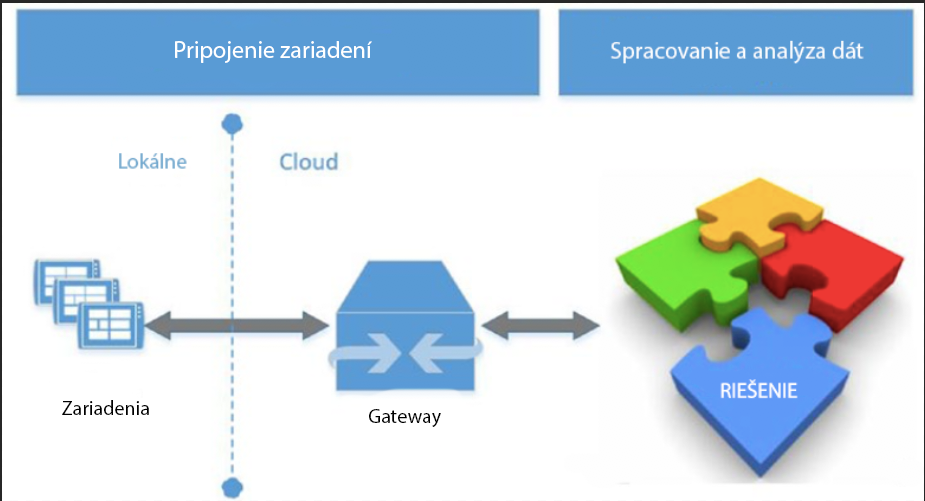
\includegraphics[width= 9.9 cm]{IoTHub1.png}
\caption{Základné náležitosti riešenia IoT  \cite{azureHub}}
\label{fig:hub1}
\end{figure}

Pripojenie zariadení predstavujú jednoducho zariadenia, ktoré generujú a zhromažďujú údaje, ktoré sa potom odosielajú do cloudovej brány. Cloudová brána funguje ako sprostredkovateľ, ktorý zhromažďuje prichádzajúce údaje a sprístupňuje ich
na ďalšie spracovanie ďalšími službami a procesmi IoT riešenia. V rámci architektúry riešení IoT však existujú skutočné a zreteľné výzvy. Tieto výzvy prichádzajú v podobe spôsobu, ako vytvoriť bezpečné a spoľahlivé spojenie medzi zariadeniami a backendovým riešením \cite{azureHub}. 
\newline

Osobitnú pozornosť treba venovať vlastnostiam, ktoré vytvárajú predstavu o skutočných výzvach, ktorým dnes čelia riešenia IoT. Sú to napríklad \cite{azureHub}:
\begin{itemize}
\item Pomalé alebo nespoľahlivé sieťové pripojenie
\item Obmedzené zdroje energie
\item Nedostatok fyzického prístupu k zariadeniu
\item Možné použitie vlastných aplikačných protokolov
\item Interakcia človeka so zariadením
\end{itemize}

Okrem toho existuje ďalšia kľúčová charakteristika zariadení, ktorú nemožno prehliadnuť. Je potrebné poznamenať, že šípka medzi zariadeniami a gateway (ako aj gateway a riešením IoT) na obrázku  \ref{fig:hub1} je obojsmerná. Je to spôsobené tým, že riešenia IoT vyžadujú bezpečnú obojsmernú komunikáciu medzi zariadeniami a cloudovými bránami.
Teda nielenže zariadenia odosielajú dáta (komunikácia zariadenie-cloud), ale môžu tiež prijímať a spracovávať správy a informácie (komunikácia typu cloud-zariadenie) z koncového bodu cloudu. Predstavte si scenár, keď by riešenie IoT mohlo odoslať zariadeniu správu s výzvou na zmenu konfiguračných hodnôt. Napríklad sa môže odoslať správa do zariadenia, ktorá mu má povedať, aby zmenil rýchlosť načítania údajov alebo zmenil horný alebo dolný limit výstrahy teploty. 
Potrebná je služba, ktorá prekoná tieto výzvy, a to nielen poskytnutím náležitej bezpečnosti a spoľahlivosti, ale v prípade potreby aj škálovateľnosťou \cite{azureHub}. 

\subsection{Komunikačné protokoly }
Na komunikáciu IoT zariadení s cloudovými platformami slúžia komunikačné protokoly. Medzi najviac používané patria CoAP, HTTP, AMQP a MQTT \cite{protocols}.
\newline

MQTT (Message Queue Telemetry Transport Protocol) je štandardizovaný transportný protokol na prenos správ na publikovanie / prihlásenie, navrhnutý pre nízku spotrebu energie, minimalizované dátové pakety a efektívnu distribúciu informácií do jedného alebo viacerých prijímačov. MQTT beží nad TCP protokolom a podporuje bezpečnú komunikáciu pomocou TLS/SSL a často sa používa v prípadoch použitia IoT \cite{protocols}.
\newline

CoAP (Constrained Application Protocol) je protokol podporujúci architektúru požiadavka / odpoveď, ako aj zdroj / pozorovanie. Je navrhnutý tak, aby umožnil jednoduchým obmedzeným zariadeniam pripojiť sa k IoT aj prostredníctvom obmedzených sietí s nízkou šírkou pásma a nízkou dostupnosťou. Spravidla sa používa na aplikácie typu stroj na stroj (M2M), ako sú inteligentná energia a automatizácia budov. Je vyvinutý hlavne na spoluprácu s HTTP a RESTful webom pomocou jednoduchých proxy serverov. Používa UDP transportný protokol a DTLS na zabezpečenie. V sieti s veľkým preťažením alebo obmedzenou konektivitou môže CoAP pokračovať v práci tam, kde protokoly založené na TCP, ako napríklad MQTT, nedokážu vymieňať informácie a efektívne komunikovať \cite{coap}.
\newline

HTTP je prevažne protokol webových správ podporujúci RESTful webovú architektúru požiadavka / odpoveď. HTTP používa TCP ako predvolený transportný protokol a TLS/SSL na zabezpečenie. HTTP sa v IoT používa obmedzene kvôli jeho nízkemu výkonu, synchrónnej komunikácií, či vysokej spotrebe energie \cite{protocols} \cite{http}.
\newline

AMQP je skratka pre Advanced Message Queuing Protocol je protokol aplikačnej vrstvy pre zasielanie správ. Obsahuje súbor štandardov, ktoré riadia celý proces zasielania správ v sprostredkovateľoch správ AMQP, ako je RabbitMQ. Umožňuje dvom stranám komunikovať odosielaním a prijímaním správ medzi nimi. \cite{rabbitmq}

\subsection{Príklady použitia}

Mnoho poskytovateľov cloudových služieb sleduje najnovšie trendy vo vývoji cloudových aplikácií a ponúka možnosti federácie na úrovni platformy, čím vytvárajú riešenia platformy ako služby (PaaS). PaaS je úplné prostredie pre vývoj a nasadenie v cloude, ktoré poskytuje prostriedky umožňujúce dodať čokoľvek od jednoduchých cloudových aplikácií po prepracované podnikové aplikácie s podporou cloudu. Neustále rastie počet poskytovateľov ponúkajúcich služby špecifické pre IoT, pretože cloud computing má potenciál uspokojiť potreby IoT, ako je skrytie úloh generovania, spracovania a vizualizácie údajov \cite{PaaS} \cite{iotcloud}.
V nasledujúcej tabuľke bude spomenutých niekoľko poskytovateľov cloudovej služby a ich využívané komunikačné protokoly.
\begin{table}[H]
\caption{Poskytovatelia IoT cloudových služieb a ich používané protokoly \cite{iotcloud}}
\begin{center}
\begin{tabular}{|c|c|}
\hline
Poskytovateľ & Protokoly \\
\hline
Bluemix & MQTT \\
Parse & HTTP \\
Google & HTTP \\
Azure & MQTT, AMQP, HTTP \\
Heroku & MQTT \\
\hline
\end{tabular}
\end{center}
\label{default}
\end{table}%

\subsubsection{IBM Bluemix Platform} 
IBM Bluemix Platform je riešenie PaaS, s podporou IoT ponúkané spoločnosťou IBM. Môže sa použiť na rýchly vývoj cloudových aplikácií, ktoré využívajú dáta generované senzormi a zariadeniami. Podporované sú produkty niekoľkých významných výrobcov zariadení, ako napríklad ARM, Electronics B\&B, Intel, Multi-Tech Systems a Texas Instruments, ale na platforme je možné vyriešiť aj ďalšie jednotlivé prípady. Dáta generované zariadením sa odosielajú do cloudu populárnym protokolom MQTT. Táto služba umožňuje používateľom konfigurovať, spravovať zariadenia a ukladať históriu generovaných údajov alebo streamovať údaje v reálnom čase do aplikácie. Prenos dát je možné vykonať prostredníctvom zabezpečených verejných rozhraní.
Platforma Bluemix ponúka niekoľko špecializovaných služieb na podporu vývoja cloudových aplikácií. Niektoré príklady týchto služieb sú: Push for messaging, Cloudant NoSQL DB na správu databáz NoSQL, Geospatial Analytics na sledovanie polohy a IBM Analytics for Hadoop pre výpočty Hadoop. Podporované jazyky pre vývoj aplikácií sú Java, JavaScript, GO, PHP, Python a Ruby  \cite{iotcloud}.

\subsubsection{Parse} 
Platforma Parse vyvinutá spoločnosťou Facebook má tiež podporu internetu vecí. Táto platforma sľubuje rýchly a ľahký vývoj aplikácií s podporou mobilných zariadení (prostredníctvom služby MBaaS). Okrem C SDK pre Linux (Raspberry Pi) a systémov v reálnom čase (RTOS) (TI CC3200) sú v ponuke aj niektoré ďalšie špeciálne verzie, ako napríklad Arduino, a množstvo partnerov má SDK, ako sú Atmel, Broadcom, Intel a Texas Instruments. Veľkou výhodou platformy je, že všetky ich súpravy SDK sú open source. Tieto SDK umožňujú odosielanie dát a takzvané push notifikácie a môžu tiež využívať výhody cloudových služieb Parse. Na demonštráciu jeho použitia je k dispozícii veľa ukážkových aplikácií vrátane scenárov poľnohospodárstva, hudby a varenia. Sú podporované javascriptové aplikácie a služba Parse Webhook umožňuje prepojenie aplikácií zo vzdialených cloudov. Podporované mobilné platformy sú iOS, Windows Phone, Android, Unity a Xamarin. Webové a desktopové SDK sú určené pre OSX, Windows, JavaScript, Unity, PHP a. NET. Je možné naplánovanie úloh, rovnako ako je k dispozícii aj vysoko kvalitný informačný panel, ktorý podporuje úpravu údajov, štatistické testovanie, push notifikácie a ukladanie logov  \cite{iotcloud}.

\subsubsection{Google Cloud Platform } 
Riešenie Google IoT je súčasťou platformy Google Cloud Platform, ktorá obsahuje rôzne služby Google. Škálovateľnosť je vynikajúcou vlastnosťou tejto platformy. Umožňuje pripojenie zariadení, zhromažďuje údaje a vizualizuje ich. Platforma IoT služby Google Cloud umožňuje automaticky predpovedať, kedy zariadenie potrebuje údržbu, a optimalizovať jeho výkon v reálnom čase, zatiaľ čo zisťuje anomálie a sleduje status, stav a polohu zariadenia. Taktiež prináša novú úroveň inteligencie a automatizácie do celých domov, budov alebo miest vytvorením komplexného riešenia, ktoré pokrýva miliardy senzorov a okrajových zariadení.
Dáta odoslané zo zariadení prijíma Google Load Balancer a ďalej ich posiela do inštancií aplikácií AppEngine. Všeobecne je hlavnou časťou aplikácie AppEngine, ktorá môže využívať ďalšie služby. Compute Engine podporuje úlohy náročné na výpočty. Cloud Storage a Cloud SQL spravujú údaje. Je možné posielať dáta pomocou streamov do služby BigQuery, čo je ideálne, ak chceme pracovať s dátami v reálnom čase. V systémoch IoT je vizualizácia dôležitou vlastnosťou, je podporovaná v reálnom čase pomocou grafov Google. Google je tiež silný v správe veľkého množstva spracovania údajov, čo je dôležité, pretože v systémoch IoT existuje veľa zariadení generujúcich obrovské množstvo údajov. Google FireBase hrá dôležitú úlohu pri správe zariadení. Pôvodne bol navrhnutý na pomoc mobilným zariadeniam (napríklad MBaaS). Poskytuje synchronizovanú databázu v reálnom čase, autentifikáciu a schopnosť offline operácií  \cite{iotcloud} \cite{google}.

\subsubsection{Azure IoT Hub } 
Azure je cloudová výpočtová platforma od spoločnosti Microsoft, ktorá umožňuje vývojárom publikovať webové aplikácie bežiace na rôznych frameworkoch napísané v rôznych programovacích jazykoch, ako sú napr. NET jazyk, Node.js, PHP, Python a Java. Komponent týkajúci sa internetu vecí sa volá IoT Hub, ktorá umožňuje obojsmernú komunikáciu medzi zariadeniami IoT a cloudovými backendovými službami pri zohľadnení všetkých bezpečnostných požiadaviek. Cloud odosiela správy do zariadení v zmysle príkazov alebo notifikácií. Príkazy sú objednávky zariadeniam na vykonávanie akcií, zatiaľ čo notifikácie sú informácie potrebné v niektorých prípadoch počas životného cyklu vykonávania niektorých príkazov. Pre každý odosielaný príkaz by cloudový backend mal dostávať spätnú väzbu od zariadenia ako potvrdzujúcu správu o úspešnom doručení alebo správu o chybe doručenia, ktorá upozorní na stav zlyhania doručenia. Podobne zariadenia odosielajú správy do cloudového backendu v dvoch formátoch, a to telemetrické údaje alebo výsledok príkazov. Azure IoT Hub má register identít na uchovávanie identity a informácií súvisiacimi s autentifikáciou každého zariadenia. Má tiež jednotku na správu všetkých pripojených a autentifikovaných zariadení. Azure IoT Hub 
\newline

Kľúčovým prvkom a jednou z výziev je, ako sa môžu zariadenia IoT pripájať k riešeniam IoT. V prípade Azure IoT Hub sa môžu zariadenia pripájať priamo alebo nepriamo. Obrázok \ref{fig:connectivity} zobrazuje tok logickej komunikácie z rôznych typov zariadení do IoT Hub. Veľkou výhodou je široké použitie komunikačných protokol ako sú MQTT, AMQP, HTTP, či použitie vlastného protokolu  \cite{azureHub} \cite{IoTHub}.

\begin{figure}[H]
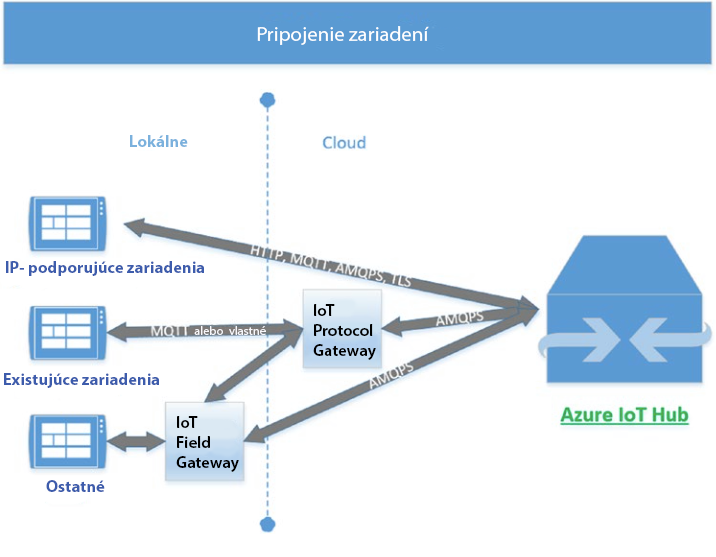
\includegraphics[width=\linewidth]{IoTHub3.png}
\caption{IoT Hub pripojenie zariadení \cite{azureHub}}
\label{fig:connectivity}
\end{figure}



\subsubsection{Heroku}
Heroku je vo vývoji od roku 2007, počnúc podporou Ruby a v priebehu rokov pridávajúc podporu mnohých jazykov, ako sú Java, Node.js, Scala, Python, PHP a Perl. Heroku získala spoločnosť Salesforce.com v roku 2010 ako dcérska spoločnosť. Služby Heroku bežia na cloudových systémoch Amazon. Z pohľadu Developer Experience je rozhranie Heroku intuitívne a ľahko použiteľné. Heroku bolo mnohokrát považované za príklad inými poskytovateľmi PaaS kvôli ich ľahkému použitiu, vlastnostiam a spoľahlivosti. V IoT Heroku ponúka doplnok CloudMQTT, ktorý slúži ako cloudový sprostredkovateľ MQTT pre IoT aplikácie. CloudMQTT slúži ako jedno z riešení pre zasielanie správ medzi snímačmi nízkej spotreby alebo mobilnými zariadeniami, ako sú telefóny, zabudované počítače alebo mikrokontroléry, ako je Arduino \cite{iotcloud} \cite{heroku}.

\section{Komunikačné technológie}

Medzi hlavné komunikačné technológie inteligentných domácností patria siete pripojiteľné k hlavnému zdroju napájania - drôtové siete ako je HomePlug, či Ethernet a bezdrôtové siete, medzi ktoré radíme napríklad Wifi, ZigBee alebo Bluetooth.

\subsection{Drôtová sieť }

V súčasnosti existuje množstvo prenosových infraštruktúr pre drôtovú sieť ako telefónne linky, optické vlákna, koaxiálne káble, či elektronické vedenie.
\newline

Komunikačná technológia elektrického vedenia s názvom HomePlug, využíva na komunikáciu  existujúce domáce elektrické vedenie. Je široko používaná pre vysokorýchlostnú
drôtovú komunikácie \cite{comunication}.
\newline

Ethernet je veľmi často používaná technológia a podporuje celý rad prenosových rýchlostí pomocou netienených krútených párov (10 Mbps-1Gbps) alebo optických vlákien (až 10Gbps). Využíva bežné rozhranie ktoré sa nachádza v zariadeniach ako sú notebooky, tlačiarne, servery, herné konzoly. Ethernet však nie je najvhodnejší na pripojenie všetkých zariadení domácej siete, vzhľadom na vysoké náklady, požiadavky na napájanie a potrebe samostatnej kabeláže späť do centrálneho bodu \cite{comunication}. 
\newline

X10 je technológia (a medzinárodný a otvorený priemyselný štandard), ktorá využíva elektrické vedenie na signalizáciu a riadenie domácich zariadení, kde signály zahŕňajú krátke vysokofrekvenčné záblesky predstavujúce digitálne informácie. Táto technológia zahŕňa aj niektoré problémy, ako je napríklad rušenie, nekompatibilita s inštalovanými spotrebičmi, pomalá rýchlosť a nedostatočné šifrovanie \cite{comunication}.
\newline

Všetky vyššie zmienené technológie dokážu komunikovať prostredníctvom IP protokolu, preto sú ľahko integrovateľné k inteligentným sieťam založených na IP protokole.
\newline

\subsection{Bezdrôtová sieť }

V dnešnej dobe je široká ponuka bezdrôtových technológií. Možno si vybrať z technológií napájaných na batériu alebo technológií využívajúcich iný zdroj energie (veterná, solárna...). Medzi široko používané bezdrôtové technológie v inteligentných domácnostiach patria Bluetooth, ZigBee, WiFi a iné.
\newline

Wi-fi je veľmi populárna bezdrôtová technológia pracujúca na frekvenčnom pásme 2,4 GHz a 5 GHz, založená na IP protokole. Používa sa v domácich sieťach, tabletoch, mobilných telefónoch a iných elektronických zariadeniach \cite{comunication}. Výhodami je jeho vysoká prenosová rýchlosť, má široké pokrytie a silnú odolnosť proti rušeniu. Oproti káblovej sieti má lepšiu škálovateľnosť a mobilitu \cite{wifi}.
\newline

ZigBee je štandard, ktorý definuje sadu komunikačných protokolov pre bezdrôtové siete krátkeho dosahu s krátkym dosahom a nízkou rýchlosťou. Zariadenia založené na Zigbee štandarde pracujú vo frekvenčných pásmach 868 MHz, 915 MH a 2,4 GHz.
ZigBee sa zameriava hlavne na aplikácie, ktoré požadujú dlhú výdrž batérie, či nízky dátový tok. To znamená, že ZigBee nepatrí k najlepšej voľbe pre implementáciu bezdrôtového internetového pripojenia. Veľa zariadení používajúcich tento štandard je väčšinu času v úspornom režime, inak povedané aj v spiacom móde. Veľkým plusom je, že zariadenia podporujúce ZigBee môžu bežať niekoľko rokov, kým nedôjde k nutnosti výmeny batérie. ZigBee umožňuje široké nasadenie v aplikáciách bezdrôtového ovládania a monitorovania \cite{zigbee}. Jednou zo ZigBee aplikácií je domáce sledovanie pacientov pri sledovaní krvného tlaku, či srdcovej frekvencie. Tieto dáta sú bezdrôtovo odosielané do lokálneho serveru pacienta, kde sa vykoná počiatočná analýza a nakoniec sú životne dôležité informácie zasielané lekárovi pacienta prostredníctvom internetu \cite{health}. 
\newline

Z-Wave je patentovaná bezdrôtová komunikačná technológia navrhnutá malou dánskou spoločnosťou s názvom Zensys, špeciálne na aplikácie diaľkového ovládania v obytných priestoroch. Z-Wave je ľahko zabudovateľný do výrobkov spotrebnej elektroniky vrátane batériových zariadení, ako sú diaľkové ovládače. Používa sa na svietenie svetiel, automatické odomykanie dverí, či bezpečnostné systémy. Výhoda Z-Wave je aj to, že jeho siete zvládnu až 232 pripojených zariadení. Z-Wave predstavuje konkurenciu pre ZigBee, avšak Z-Wave získal podporu čipového giganta Intel a taktiež sieťovej firmy Cisco. ZigBee a Z-Wave sú ale v mnohých veciach veľmi podobné technológie \cite{z-wave}. 
\newline

Všetky vyššie zmienené typy bezdrôtových sietí patria medzi nízkonákladové siete a siete s nízkym výkonom (napájané z batérie) \cite{comunication}.
\newline

Bluetooth patrí do skupiny štandardov IEEE 802.15.1. Jeho vývoj začal koncom roku 1998 keď spoločnosti Ericsson, IBM, Intel, Nokia a Toshiba vytvorili skupinu Bluetooth Special Industry Group (SIG). Cieľom bolo vyvinúť globálne riešenie bezdrôtovej komunikácie krátkeho dosahu, fungujúce v bezlicenčnom pásme 2,4 GHz (ISM - Industrial-Scientific-Medical band). Ide taktiež o nízkonákladovú technológie, ako aj technológie už vyššie spomenuté \cite{bluetooth}. 
Komunikačné nástroje s nízkou energetickou spotrebou sú budúcnosťou IoT. Preto za zmienku stojí aj Bluetooth Low Energy (BLE) ide o veľmi energeticky efektívnu verziu Bluetooth (pokiaľ ide o prenesenie bajtov na jeden Joul) s relatívne krátkym dosahom (50 m), komunikujúca nad protokolom IPv6. BLE sľubuje, že senzory budú schopné komunikovať pomocou gombíkovej batérie dokonca až dva roky \cite{ble} \cite{casio}.
\newline

EnOcean je bezdrôtová komunikačná technológia s veľmi nízkym výkonom, ktorá na svoje fungovanie využíva energiu získavanú z okolia, napríklad premenou tepelnej, elektromagnetickej alebo solárnej energie na elektrickú. Je energeticky účinnejšia ako iné bezdrôtové komunikačné technológie, ako sú Zigbee a Bluetooth. Benefitmi produktov založených na princípe EnOcean sú hlavne znížené náklady na inštaláciu a údržbu.
EnOcean sa stal štandardom v roku 2012 (ISO/IEC 14543-3-10). Tento štandard pokrýva vrstvy 1-3 OSI modelu, a to fyzickú, linkovú a sieťovú. Vlastníkom patentu je spoločnosť EnOcean, založená ako spin-off spoločnosťou Siemens AG. Cieľom EnOcean bolo vyvinutie bezdrôtových modulov, ktoré dokážu napájať sami seba bez potreby pridania batériového zdroja.
EnOcean využíva viaceré transportné frekvencie. Konkrétne 902 MHz, 928,35 MHz a 315 MHz.
Rádiové signály z EnOcean senzorov a spínačov je možné prenášať bezdrôtovo na vzdialenosť až 300 metrov v otvorenom priestore a až 30 metrov vo vnútri budov \cite{enocean}\cite{enoceancvut}. 
\newline

\begin{figure}[H]
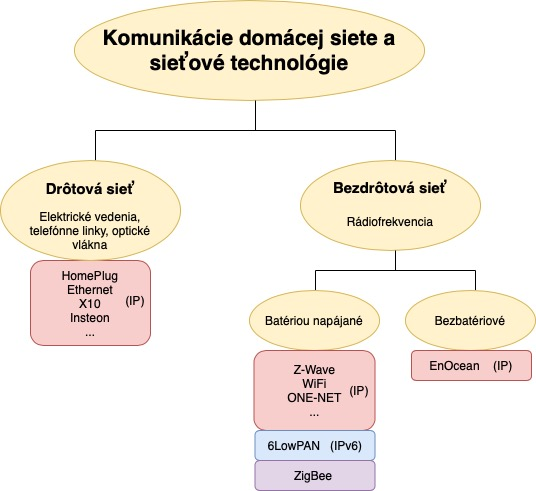
\includegraphics[width=\linewidth]{diagram-2.jpg}
\caption{Komunikácia domácej siete a sieťové technológie \cite{comunication}}
\label{fig:net}
\end{figure}

\section{Technológia inteligentných domácich sietí} 
Technológia inteligentných domácich sietí je k dispozícii v troch hlavných oblastiach: Powerline (X10, EIB Powerline), Busline: EIB, Cebus, Lonwork, Batibus EHS ) a vysokofrekvenčné (RF) (napr. Bluetooth a väčšina významných výrobcov inteligentných domov)  \cite{networks}.

\subsection{Powerline}
Systémy Powerline sa skladajú zo zariadení, ktoré je možné pripojiť priamo k hlavnému zdroju napájania. Tieto zariadenia používajú bežné vedenie na zasielanie údajov do zariadení, aby ich aktivovali alebo deaktivovali. Technológia Powerline je ľahko konfigurovateľná a systém môže byť v prevádzke rýchlo a lacno. Powerline systémy vyžadujú pripojenie k počítaču k monitorovaniu zariadenia alebo zmene ich stavu. V novších systémoch v prípade použitia kódovania X10 je možné obísť potrebu pripojenia k počítaču umiestením čipových sád do systému. Najväčší problém u týchto systémov môže nastať pri výpadku alebo prerušení napájania  \cite{networks}.

\subsection{Busline}
Inteligentné domy Busline používajú na prenos dát do zariadení samostatný 12-voltový kábel (krútený pár), ktorý je paralelný s tradičným sieťovým káblom. Tým sa zabezpečuje nezávislosť na bežnom sieťovom zdroji napájania. Busline sa javí ako najefektívnejšia a najspoľahlivejšia forma inteligentných domácností, pretože je možné ju nakonfigurovať tak, aby zabránila poruchám zariadení počas výpadkov napájania  \cite{networks}.

\subsection{Bezdrôtové siete}
Dnes si získavajú popularitu hlavne vysokofrekvenčné (RF) a infračervené (IR) systémy. Mnoho výrobcov používa vo svojich produktoch práve RF systém. Avšak tieto produkty majú problém s interferenciou a problémami s identifikáciou krátkeho dosahu.
RF systémy boli kritizované, pretože by do nich mohol preniknúť votrelec so správnym IR kódom, ktorý by mohol získať prístup do domácnosti alebo upraviť nastavenia zariadení  \cite{networks}.
\newline

\section{Bezpečnosť} 
Inteligentná domácnosť je najrýchlejšie rastúcou oblasťou technológie internetu vecí. Vďaka pripojeniu na internet, dynamickej a heterogénnej povahe vytvára inteligentná domácnosť nové bezpečnostné problémy a výzvy. V nasledujúcich podkapitolách popisujeme najdôležitejšie ciele bezpečnosti inteligentnej domácnosti, útoky na bezpečnosť a možné hrozby \cite{securitytitle}.

\subsection{Ciele bezpečnosti}
Šesť najdôležitejších cieľov pre zabezpečenie inteligentnej domácnosti sú \cite{security}:
\begin{itemize}
\item Dôvernosť: záruka, že údaje budú zverejnené iba oprávneným osobám alebo systémom.
\item Integrita: záruka, že sa zachová presnosť a konzistentnosť údajov. Žiadne neoprávnené úpravy, zničenie alebo straty údajov nezostanú neodhalené.
\item Dostupnosť: záruka, že akýkoľvek sieťový zdroj (dáta / šírka pásma / zariadenie) bude vždy k dispozícii pre akýkoľvek autorizovaný subjekt. Takéto zdroje sú tiež chránené pred akýmikoľvek incidentmi, ktoré ohrozujú ich dostupnosť.
\item Autenticita: potvrdenie, že komunikujúce strany sú tým, za koho sa vydávajú, a že správy, ktoré údajne odosielajú, skutočne odosielajú oni.
\item Autorizácia: záruka, že prístupové práva všetkých subjektov v systéme sú definované na účely kontroly prístupu.
\item Nepopierateľnosť: uistenie, že budú existovať nepopierateľné dôkazy na overenie pravdivosti akýchkoľvek tvrdení subjektu.
\end{itemize}


\subsection{Útoky na bezpečnosť}
Útoky na bezpečnosť v prostredí inteligentných domácností sa zvyčajne pokúšajú narušiť jeden alebo viac bezpečnostných cieľov, opísaných vyššie. Tieto útoky možno rozdeliť do dvoch kategórií.
\newline

Do prvej kategórie, konkrétne „pasívnych útokov“, zaraďujeme útoky, ktoré sa snažia získať alebo využiť informácie zo systému bez ovplyvnenia systémových prostriedkov. Inými slovami, pri pasívnych útokoch má protivník v úmysle získať prenášané informácie nie preto aby ich upravoval, ale preto aby sa z nich niečo naučil. Pasívne útoky môžu mať formu odpočúvania alebo analýzy dopravy. Odpočúvaním sa rozumie neoprávnené odpočúvanie prebiehajúcej komunikácie bez súhlasu komunikujúcich strán. Analýzou prenosu označujeme niečo jemnejšie. V analýze prenosu protivník nezachycuje konkrétny obsah správy ako pri odpočúvaní, ale sleduje vzorce prenosu, aby z nich odvodil užitočné informácie. Oba tieto útoky sa považujú za ťažko odhaliteľné, pretože nemenia údaje. Pri ich riešení sa teda zameriavame skôr na prevenciu ako na detekciu  \cite{security}.
\newline

Druhú kategóriu tvoria „aktívne útoky“, do ktorej umiestňujeme útoky, ktoré sa snažia zmeniť systémové prostriedky alebo ovplyvniť jeho fungovanie. Aktívne útoky môžu zahŕňať určité úpravy údajov alebo zavedenie podvodných údajov do systému. Najbežnejším útokom je maskovanie, útok z opakovaného prehrávania, zmena správy, odmietnutie služby (DoS) a škodlivý softvér. K maskujúcemu útoku dôjde, keď sa votrelec vydáva za legitímnu entitu, ktorá získa privilégiá. Útok z opakovaného prehrávania zahŕňa pasívne zachytenie správ v komunikácii a ich opakovaný prenos, ktorý má neautorizovaný efekt. Útok na zmenu správy zahŕňa zmenu obsahu legitímnej správy, oneskorenie alebo zmenu poradia toku správ s cieľom vyvolať neoprávnený účinok. Cieľom útoku odmietnutia služby je dočasné alebo trvalé prerušenie alebo pozastavenie dostupnosti komunikačných prostriedkov systému. Napokon útoky škodlivého softvéru znamenajú útoky zamerané na zneužitie vnútorných chýb zabezpečenia na úpravu, zničenie a odcudzenie informácií alebo na získanie neoprávneného prístupu k systémovým prostriedkom \cite{security}.
\newline

\subsection{Hrozby}
Inteligentné domácnosti sú pre spotrebiteľov čoraz atraktívnejšie a pravdepodobne sa o niekoľko rokov stanú populárnymi a budú súčasťou bežného života. 
Systém teda bude musieť odolávať rôznym hrozbám. Niektoré z nich budú popísané nižšie.
\newline

Jedna z možných hrozieb na útok bezpečnosti inteligentnej domácnosti je už existujúca hrozba na počítače a mobilné zariadenia v podobe malware. Ide predovšetkým o škodlivý softvér, ktorý sa snaží získať prihlasovacie údaje alebo iné informácie. Vzhľadom na to, že niektoré zo zariadení inteligentnej domácnosti sú malé počítače, je táto hrozba možným problémom. V súčasnosti malware dokáže šifrovať súkromné dokumenty, a za ich dešifrovanie sú požadované peniaze. Malware môže spôsobiť nemalé problémy v zariadeniach inteligentných domácností, keď nad nimi prevezme kontrolu a napríklad svetlá budú vypnuté, dvere uzamknuté, či deaktivované kúrenie. Súkromný dom sa tak stane rukojemníkom cudzej osoby. V súčasnosti je bežná domácnosť vybavená priemerne jedným routrom, no v budúcnosti môže mať mnoho zariadení inteligentnej domácnosti \cite{threats}.
\newline

Ďalšia hrozba prichádza so samotným votrelcom. Vďaka bezdrôtovým zariadeniam a monitorovacím systémom mohli zlodeji pomocou nechránených alebo nezabezpečených systémov inteligentných domácností hľadať svoje obete a skryť svoju vlastnú prítomnosť. Najskôr špehujú ľudí a keď nebudú doma, potom simulujú nedotknutý domov a zároveň kradnú nájdené poklady \cite{threats}.
\newline

Ďalšou možnou hrozbou je preniknutie do najslabšieho článku všetkých zariadení pripojených k internetu a pomocou neho dokáže páchateľ preniknúť do celého systému.
Nie každé zariadenie má ale rovnakú úroveň rizika ako cieľ útoku. Niektoré zariadenia, najmä nespracované senzory, môžu mať vysoké obmedzenie pamäte a výpočtového výkonu, čo ich robí nepríťažlivými \cite{threats}.

\chapter{Požiadavky na systém}
\label{chap:requirements}

\subsection*{Denník}
\begin{enumerate}
\item Systém umožní užívateľovi registrovať sa a prihlásiť sa do aplikácie.
\item Systém umožní užívateľovi sledovať stav jeho záhrady odkiaľkoľvek s možnosťou pripojenia na internet.
\item Systém umožní užívateľovi pridať rastlinu a vyplniť údaje o tejto rastline.
\item Systém umožní užívateľovi odstrániť pestovanú rastlinu zo zoznamu rastlín.
\item Systém umožní užívateľovi upraviť minimálnu a maximálnu možnú teplotu pestovania rastliny.
\item Systém umožní užívateľovi vyhľadať rastlinu podľa názvu.
\item Systém umožní užívateľovi zobraziť históriu pestovania rastlín a počasia.
\item Systém informuje užívateľa, že skončila sezóna rastliny.
\item Systém informuje užívateľa, že začala sezóna rastliny.
\item Systém informuje užívateľa, že začalo obdobie dozrievania plodov na určitej rastline.
\end{enumerate}

\subsection*{Riadenie podmienok}
\begin{enumerate}
\item Systém bude zbierať dáta pomocou senzorov.
\item Systém umožní užívateľovi zobraziť  vlhkosť pôdy.
\item Systém umožní užívateľovi zobraziť  teplotu vzduchu. 
\item Systém umožní užívateľovi zobraziť prehľad zrážok.
\item Systém umožní užívateľovi nastaviť časový interval merania senzorov.
\item Systém umožní užívateľovi nastaviť upozornenie na požadovanú teplotu.
\item Systém umožní užívateľovi nastaviť čas pravidelného zalievania.
\end{enumerate}

\subsection*{Upozornenia}
\begin{enumerate}
\item Systém upozorní užívateľa, ak senzor nameria teplotu, požadovanú užívateľom.
\item Systém upozorní užívateľa, že v najbližších dňoch teplota klesne pod minimálnu teplotu na pestovanie určitej rastliny..
\item Systém upozorní užívateľa, ak teplota stúpne nad maximálnu teplotu na pestovanie určitej rastliny.
\item Systém upozorní užívateľa, ak teplota klesne pod minimálnu teplotu na pestovanie určitej rastliny.
\item Systém upozorní užívateľa, ak teplota klesne pod 0 °C.
\item Systém upozorní užívateľa, ak je pôda suchá.
\end{enumerate}

\subsection*{Nice to Have}
\begin{enumerate}
\item Systém umožní užívateľovi si vybrať automatické zavlažovanie, ak senzor zaznamená suchú pôdu. 
\item Systém umožní užívateľovi odstrániť svoj profil.
\item Systém umožní užívateľovi pridať fotky rastlín.
\item Systém umožní užívateľovi si vybrať medzi polievaním z kohútika a polievaním z nádrže.
\end{enumerate}

\chapter{Prieskum existujúcich riešení}
Na základe požiadaviek na systém je potrebné zaistiť softvérové a hardvérové riešenie smart záhrady. Preto sa v tejto kapitole budeme venovať prieskumu existujúcich softvérových, hardvérových, či úplných riešení smart záhrad a analyzovať ich výhody, nevýhody, cenu a cieľovú skupinu ľudí, pre ktorú sú konkrétne riešenia vhodné. Na základe tohoto prieskumu sme schopní vyskladať vhodné riešenie pre uvedené požiadavky na systém  v kapitole ~\ref{chap:requirements}.
\section{Hotové riešenia}
Pod hotovými riešeniami si môžeme predstaviť riešenia, ktoré obsahujú smart aplikáciu, senzory a zber dát z týchto senzorov, prípadne riadenie týchto senzorov.
\subsection*{FarmBot}
FarmBot je americký projekt s otvoreným zdrojom, ktorý umožňuje úpravy a doplnky hardvéru, softvéru a dokumentácie od používateľov. 
Cieľom projektu je „Vytvoriť otvorenú a prístupnú technológiu, ktorá pomôže každému pestovať jedlo a pestovať ho pre každého".
Využíva online databázu plodín s názvom OpenFarm na vytvorenie optimálneho plánu výsadby na základe veľkosti dospelých plodín.  \cite{farmbot}
\newline

\textbf{VÝHODY}
\begin{itemize}
\item open-source
\item automatické procesy sejby, mechanickej regulácie buriny, zavlažovania
\item rôzne spôsoby napájania na zdroj energie a zavlažovania
\end{itemize}

\textbf{NEVÝHODY}
\begin{itemize}
\item  absencia jazykovej mutácie
\item  obmedzenie na pestovateľskú rozlohu : 
	\begin{enumerate}
	\item 2,9 m × 1,4 m s maximálnou výškou rastliny 0,5 m
	\item 5,9 m x 2,9 m s maximálnou výškou rastliny 0,5 m
	\item 5,7 m x 2,3 m s maximálnou výškou rastliny 0,5 m
	\item 2,7 m x 1,1 m s maximálnou výškou rastliny 0,5 m
	\end{enumerate}
\end{itemize}
	
\textbf{CENA}
\begin{itemize}
\item 2.506,95 €  + 280 € doprava = $\sim$ 63 000 Kč + 7 000 Kč 
\item 4.167,95 € + 280 € doprava = $\sim$ 105 000 Kč + 7 000 Kč
\item 1.376,95 € + 280 € doprava = $\sim$ 35 000 Kč + 7 000 Kč
\item 1.247,95 € + 280 € doprava = $\sim$ 31 500 Kč + 7 000 Kč
\end{itemize}

\textbf{CIEĽOVÁ JEDNOTKA}
\begin{itemize}
\item domáce záhrady / domáci pestovatelia
\item prevažne cielené pre americký trh
\end{itemize}

\subsection*{LoDaWAN®  Agricultural Monitoring Node-to-App}
Pre uspokojenie potreby inteligentného poľnohospodárstva, spoločnosť Ursalink navrhla súpravu LoDaWAN®  Agricultural Monitoring Node-to-App. Jeho cieľom je zjednodušiť proces vzdialeného monitorovania a vybudovať dôkladnú poľnohospodársku stratégiu založenú na dátach.  \cite{lorawan}
\newline

\textbf{VÝHODY}
\begin{itemize}
\item obsahuje rozmanité druhy senzorov
\item napájanie na vlastný Ursalink cloud - rok zdarma
\item má nízku spotrebu energie, a preto nie je nutnosť napájania z elektrickej siete
\item automatické zavlažovanie
\end{itemize}

\textbf{NEVÝHODY}
\begin{itemize}
\item absencia jazykovej mutácie
\item nutnosť širokého pokrytia siete
\end{itemize}
	
\textbf{CENA}
\begin{itemize}
\item 740 €  = $\sim$ 20 000 Kč 
\end{itemize}

\textbf{CIEĽOVÁ JEDNOTKA}
\begin{itemize}
\item veľkí poľnohospodári
\end{itemize}


\subsection*{Klarstein GrowIt Farm}
Klarstein GrowIt Farm je inteligentný kvetináč, ktorý slúži na zjednodušenie pestovania rastlín, hlavne byliniek, pre pestovateľov, ktorí nemajú vlastnú záhradu.  \cite{klarstein}
\newline

\textbf{VÝHODY}
\begin{itemize}
\item pestovanie bez pôdy
\item pestovanie bez pesticídov
\item automatické ovládanie svetla, automatické zavlažovanie
\item optický alarm pri príliš nízkej hladine živného roztoku
\end{itemize}

\textbf{NEVÝHODY}
\begin{itemize}
\item obmedzená kapacita priesad - 28 priesad na jednu sadu
\item obmedzenie na rozmery pestovaných rastlín
\item nutnosť výmeny živného roztoku a špongií pre pestovanie nových priesad
 \end{itemize}

\textbf{CENA}
\begin{itemize}
\item 250 €  =  $\sim$ 6 300 Kč 
 \end{itemize}

\textbf{CIEĽOVÁ JEDNOTKA}
\begin{itemize}
\item interieroví pestovatelia
\end{itemize}

\subsection*{Gardena}
GARDENA zavlažovací počítač - súprava, pozostávajúca zo smart zavlažovacieho počítača, smart vstupnej brány a smart senzoru, automaticky riadi prívod vody do záhrady, a tým zaisťuje flexibilný manažment vody. \cite{gardena}
\newline

\textbf{VÝHODY}
\begin{itemize}
\item silné antény pre bezdrôtové pripojenie
\item voľba ľubovoľného dňa zavlažovania
\item český aj slovenský jazyk aplikácie
\end{itemize}

\textbf{NEVÝHODY}
\begin{itemize}
\item neobsahuje automatické zavlažovanie podľa vlhkosti pôdy
\item smart zavlažovací počítač funguje v nepretržitom režime iba 60 minút
\end{itemize}

\textbf{CENA}
\begin{itemize}
\item 300 €  =  $\sim$ 7 900 Kč 
\end{itemize}

\textbf{CIEĽOVÁ JEDNOTKA}
\begin{itemize}
\item domáce záhrady / domáci pestovatelia
\end{itemize}
 
 
\section{Čiastočné riešenia}
Sekcia čiastočných riešení obsahuje neúplné riešenia smart záhrady. Ide o aplikácie bez IoT riešenia, senzory alebo čidlá bez smart aplikácie alebo senzory, ktoré síce ponúkajú aplikáciu, ale nie je možné ich ovládať na diaľku.

\subsection{Aplikácie}
\subsubsection*{Agrivi}
Softvér na správu farmy Agrivi umožňuje plánovať, monitorovať a analyzovať všetky aktivity na farme. Spracovanie pôdy, výsadba, postrek, hnojenie, zavlažovanie, zber a všetky ďalšie činnosti sú zaznamenané v aplikácií. \cite{agrivi}
\newline

\textbf{VÝHODY}
\begin{itemize}
\item monitorovania a sledovania všetkých aktivít farmy
\item sledovanie výdavkov farmy
\item predpovede počasia
\item 3-ročná história počasia pre každé pole
\item inteligentné alarmy na detekciu rizika chorôb
\item stav zásob na sklade v reálnom čase 
\item podpora platforiem Android, iOS a ako webová aplikácia
\end{itemize}

\textbf{NEVÝHODY}
\begin{itemize}
\item pre malých pestovateľov je mnoho informácií zbytočných
\item absencia českého alebo slovenského jazyka
\item zložité nastavenie upozornení na počasie
\end{itemize}

\textbf{CENA}
\begin{itemize}
\item 19 \$ = $\sim$ 420 Kč na mesiac 
\end{itemize}

\textbf{CIEĽOVÁ JEDNOTKA}
\begin{itemize}
\item veľkí poľnohospodári / farmy
\end{itemize}


\subsubsection*{Garden Planner}
Garden Planner je aplikácia, ktorá učí pestovať rastliny na základe skúseností. Vedenie záznamu zabráni opakovaniu chýb a frustrácie nad strateným časom a priestorom. \cite{planner}
\newline

\textbf{VÝHODY}
\begin{itemize}
\item pridávanie fotografií
\item záznamy o sadení, polievaní, hnojení a zbieraní úrody
\item obsahuje databázu chorôb a škodcov
\item využíva údaje o klíme na zasielanie rád o výsadbe
\item umožní kresliť zeleninové záhradné plány
\item upozornenia e-mailom
\end{itemize}

\textbf{NEVÝHODY}
\begin{itemize}
\item neobsahuje predpoveď ani históriu počasia
\item neupozorňuje na zmenu počasia
\item absencia českého alebo slovenského jazyka
\end{itemize}

\textbf{CENA}
\begin{itemize}
\item 27 € = $\sim$ 700 Kč na rok
\end{itemize}

\textbf{CIEĽOVÁ JEDNOTKA}
\begin{itemize}
\item domáce záhrady / domáci pestovatelia
\item veľkí poľnohospodári
\end{itemize} 

\subsection{IoT senzory}

\subsubsection*{RainBird ST8-2.0 Smart Irrigation Timer}
RainBird značka ponúka rôzne modely regulátorov zavlažovania. Model ST8-2.0 Smart Irrigation Timer je inteligentný zavlažovací časovač. Obsahuje WiFi prijímač, vďaka ktorému je možné sa jednoducho pripojiť na modul. RainBird ponúka aj vlastnú aplikáciu, ktorá dokáže regulovať množstvo zavlažovania a nastavovať intervaly tohoto zavlažovania podľa sezóny, počasia, teploty, či vlhkosti. Ostatné RainBird moduly však nie sú obohatené o WiFi prijímač, avšak je možné si ho navyše dokúpiť. \cite{rainbird}
\newline

\textbf{VÝHODY}
\begin{itemize}
\item možnosť pripojenia na aplikáciu
\item možnosť manuálneho nastavenia modulu
\item aplikácia podáva mesačné správy o polievaní
\item výstrahové upozornenia
\item maximálna dĺžka polievania sú 3 hodiny
\end{itemize}

\textbf{NEVÝHODY}
\begin{itemize}
\item externý káblový zdroj napájania + záložný zdroj napájanie na 2 batérie 
\item aplikácia súvisí len so zavlažovaním
\item ponúka iba mobilnú aplikáciu 
\item aplikácia je kompatibilná iba s platformami iOS a Android
\end{itemize}

\textbf{CENA}
\begin{itemize}
\item 180  \$ = $\sim$ 4 500 Kč
\end{itemize}

\subsubsection*{Xiaomi Mi Flora Monitor}
Xiaomi Mi Flora Monitor je smart senzor pre rastliny, ktorý dokáže merať teplotu, vlhkosť pôdy, intenzitu svetla, či množstvo živín v pôde. Pre lepšie fungovanie je možné pomocou Bluetooth prepojiť senzor so smart aplikáciou Xiaomi MiHome v mobilnom telefóne. \cite{xiaomimiflora}
\newline

\textbf{VÝHODY}
\begin{itemize}
\item detektor svetla a živín
\item monitoring teploty a vlhkosti 
\item smart aplikácia so štatistikou nameraných dát
\item pripojenie k telefónu pomocou Bluetooth
\item napájanie batériou
\end{itemize}

\textbf{NEVÝHODY}
\begin{itemize}
\item monitorovanie iba jednej rastliny
\item nevykonáva zavlažovanie
\item absencia českého alebo slovenského jazyka
\end{itemize}

\textbf{CENA}
\begin{itemize}
\item 649 Kč
\end{itemize}

\subsubsection*{Zatvárač ventilov iQtech SmartLife}
\label{sec:agora}
Elektrický zatvárač guľových ventilov iQtech SmartLife VC01W je Smart elektrický pohon pre zatváranie a otváranie guľových ventilov vody a plynu.
Je ho možné použiť na štandardné pákové ventily pre vodu a plyn ako v domácnosti, tak aj na záhrade. Obdobné lacnejšie neznačkové smart zatvárače ponúkajú rôzne iné internetové obchody. \cite{agora}
\newline

\textbf{VÝHODY}
\begin{itemize}
\item odolný teplotám od -25 °C do +85 °C
\item pripojiteľné priamo na vodovodný kohútik
\item pripojenie k zariadeniu pomocou Wi-Fi
\item rýchle zatváranie a otváranie ventilu
\item pripojiteľné na smartlife aplikáciu pre ovládanie z telefónu
\item možnosť pripojenia k asistentom Apple Siri, Amazon Alexa, či Google Home
\end{itemize}

\textbf{NEVÝHODY}
\begin{itemize}
\item externý káblový zdroj napájania
\item iba otáčanie ventilu
\end{itemize}

\textbf{CENA}
\begin{itemize}
\item 84 € = $\sim$ 2100 Kč
\end{itemize}

\subsection{IoT riešenia pomocou mikrokontroléra}

\subsubsection*{Espressif Systems ESP8266 } 
\label{sec:esp}
ESP8266 je lacný mikročip Wi-Fi s úplným protokolom TCP / IP a mikrokontrolérom, ktorý vyrába spoločnosť Espressif Systems v čínskom Šanghaji. Slúži primárne ako mikročip pre vytváranie IoT aplikácií. Obsahuje 32-bitový Tensilica procesor, ktorý vďaka Real-Time Operating System (RTOS) a Wi-Fi stack umožňujú, aby asi 80\% procesného výkonu bolo k dispozícii pre programovanie a vývoj používateľských aplikácií v Arduine. Modul podporuje technológiu OTA (On The Air), ktorá umožňuje nahrávanie programu aj firmwéru cez bezdrôtovú sieť wifi. Samotné ESP8266 pri kúpe neposkytuje žiadne senzory, avšak je možné si ich dokúpiť veľmi lacno. \cite{conclusionSolution} \cite{esp}
\newline

\textbf{VÝHODY}
\begin{itemize}
\item vhodný do priemyselného prostredia
\item odolný teplotám od -40 °C do +125 °C
\item obsahuje výkonný zosilňovač a nízkošumový prijímač zosilňovača
\item extra nízka spotreba energie
\item architektúra šetriaca energiu (aktívny režim, režim spánku, režim hlbokého spánku)
\item programovateľný cez USB
\item prevádzkové napätie 3.3V
\item programovateľný jazykmi C, C++ a Wiring platformou
\end{itemize}

\textbf{NEVÝHODY}
\begin{itemize}
\item melé množstvo pinov pre pripojenie senzorov 
\item prevádzková pamäť <45kB
\end{itemize}

\textbf{CENA}
\begin{itemize}
\item 5-7 € = $\sim$ 125-175 Kč
\end{itemize}

\subsubsection*{Arduino}
Doska arduino je voľne dostupný vývojový open-source mikrokontrolér, schopný vyrovnať sa s rôznymi komunikačnými protokolmi, ktoré musia byť použiteľné pre akýkoľvek druh IoT zariadení. Táto doska je lacná a na funkcie bohatá dostupnosťou rôznych dcérskych dosiek. Dostupnosť wifi a ethernetu spolu s nízkym výkonom BLE-4, ho robí vhodným pre rýchle prototypy a ľahké programovanie. Samotné Arduino pri kúpe neposkytuje žiadne senzory, avšak je možné si ich dokúpiť veľmi lacno. \cite{conclusionSolution} \cite{arduino} \cite{prosconsArduino}
\newline

\textbf{VÝHODY}
\begin{itemize}
\item ethernet pripojenie
\item knižnica príkladov už s hotovým kódom
\item automatická konverzia jednotiek
\item programovateľný cez USB
\end{itemize}

\textbf{NEVÝHODY}
\begin{itemize}
\item systémová pamäť 2 kB
\item prevádzkové napätie 5V
\item programovateľný Wiring platformou
\end{itemize}

\textbf{CENA}
\begin{itemize}
\item 20 € = $\sim$ 500 Kč
\end{itemize}

\subsubsection*{Raspberry Pi}
Rasberry Pi je využiteľný na rôzne spôsoby. Napríklad ako malý stolný počítač, smart home hub, kontrolér továrne, či ako mozog robota. Zabudované wifi, BLE, úložná kapacita tejto dosky a dostupná RAM, ktorá je v porovnaní s ostatnými doskami veľmi veľká, jej umožňuje fungovať ako server IoT vo väčšine konfigurácií siete IoT. Samotné Raspberry Pi pri kúpe neposkytuje žiadne senzory, avšak je možné si ich dokúpiť veľmi lacno. \cite{conclusionSolution} \cite{raspberryPi}
\newline

\textbf{VÝHODY}
\begin{itemize}
\item ARM technológia
\item väčšie množstvo pinov pre pripojenie senzorov
\item ethernet pripojenie
\item výber veľkostí RAM
\item programovateľný jazykmi C, python, Java, Scratch, Ruby
\item systémová pamäť 1 GB
\end{itemize}

\textbf{NEVÝHODY}
\begin{itemize}
\item prevádzkové napätie 5V
\end{itemize}

\textbf{CENA}
\begin{itemize}
\item od 35 \$= $\sim$ 875 Kč
\end{itemize}

\chapter{Návrh riešenia}

Výsledkom navrhovaného riešenia bude existujúce hardvérové riešenie kombinované s vlastnou webovou aplikáciou. Navrhované riešenie pozostáva z mikročipu ESP8266 od spoločnosti Espressif Systems, na ktorom je napojené senzor na meranie teploty, vlhkosti vzduchu, tlaku vzduchu, vlhkosti pôdy a zrážkomer. Taktiež riadi spúšťanie senzoru na polievanie záhrady, ktorý následne spustí prívod vody k rastlinám. Namerané dáta zo senzorov sa následne odosielajú pomocou MQTT protokolu na server, ktorý pomocou JDBC uloží dáta do databázy. Backend a frontend medzi sebou komunikujú pomocou REST rozhrania.

\begin{figure}[H]
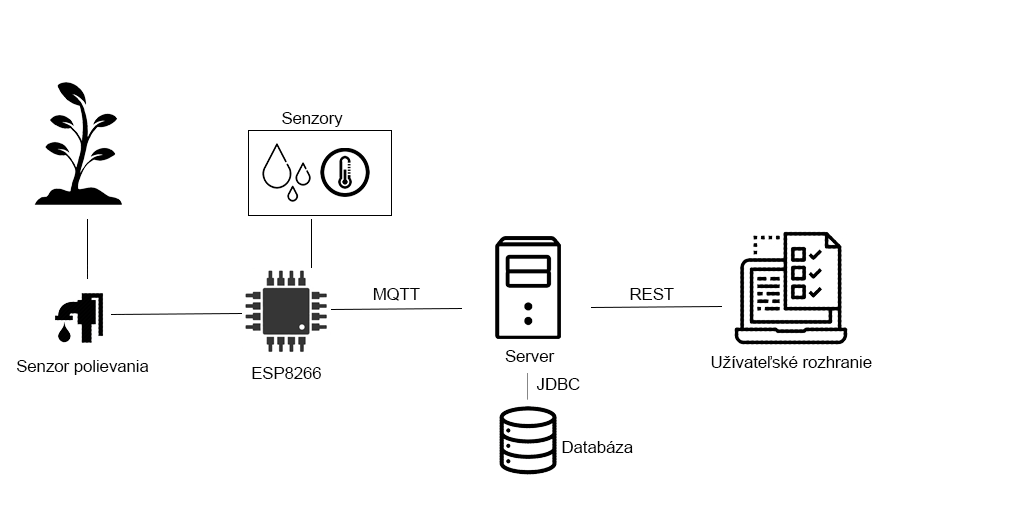
\includegraphics[width= 14 cm]{navrh.png}
\caption{Diagram navrhovaného riešenia}
\label{fig:navrh}
\end{figure}

\section{Hardvér}
 Súčasťou hardvérového riešenia je mikročip ESP8266, ktorý je podrobne popísaný v sekcií ~\ref{sec:esp}. Dôvod výberu bola ponuka vybavenia modulu, možnosť vlastného naprogramovania riadenia senzorov a cena. Senzor na meranie teploty, vlhkosti pôdy a zrážkomer bol vybraný z dôvodu potreby spracovávať dáta spojené s vlastnosťami týchto senzorov. Na riešenie polievania záhrady je použitý ventilový kontrolér pre otáčanie ventilu, podrobnejšie spomenutý v predchádzajúcej kapitole, v sekcií ~\ref{sec:agora}, na zatváranie kohútika pre reguláciu prívodu vody. Dôvod výberu bola možnosť bezdrôtového riadenia senzoru a cena. 
 
\section{Softvér}
\label{sec:software}
Softvérové riešenie pozostáva z kombinácie backendovej a frontendovej aplikácie.
Na server sa budú posielať dáta namerané senzormi pomocou protokolu MQTT. MQTT komunikácia bola vybraná z dôvodu vysokej použiteľnosti v IoT projektoch a pre nízku spotrebu energie. 

\subsection{Backend}
Backendová aplikácia bude napísaná v jazyku Java a bude služíť na spracovanie dát a ich ukladanie do databázy pomocou JDBC. Jazyk Java pre backendovú aplikáciu bol zvolený kvôli mojim najväčším skúsenostiam v tomto jazyku.

\subsection{Frontend}
Frontendovou aplikáciou bude javascriptová aplikácia, ktorá bude slúžiť ako užívateľské rozhranie. Dôvodom výberu jazyka JavaScript a nie JavaServer Pages bola možnosť využívať moderné technológie, ako sú modálne okná.  Aplikácie budú medzi sebou komunikovať pomocou REST rozhrania. To dovoľuje jednoduchý prístup k zdrojom vďaka CRUD metódam. Užívateľské rozhranie bude ponúkať informácie o teplote, vlhkosti vzduchu a pôdy, možnosť pridať informácie o svojich pestovaných rastlinách a bude ponúkať ovládanie jednotlivých senzorov.

\subsection{Databáza}
Dáta budú ukladané do databázy PostgreSQL. Dôvod výberu bola dobrá odozva na chyby, prehľadnosť a vyspelosť databáze.

\section{Diagram tried}
\begin{figure}[H]
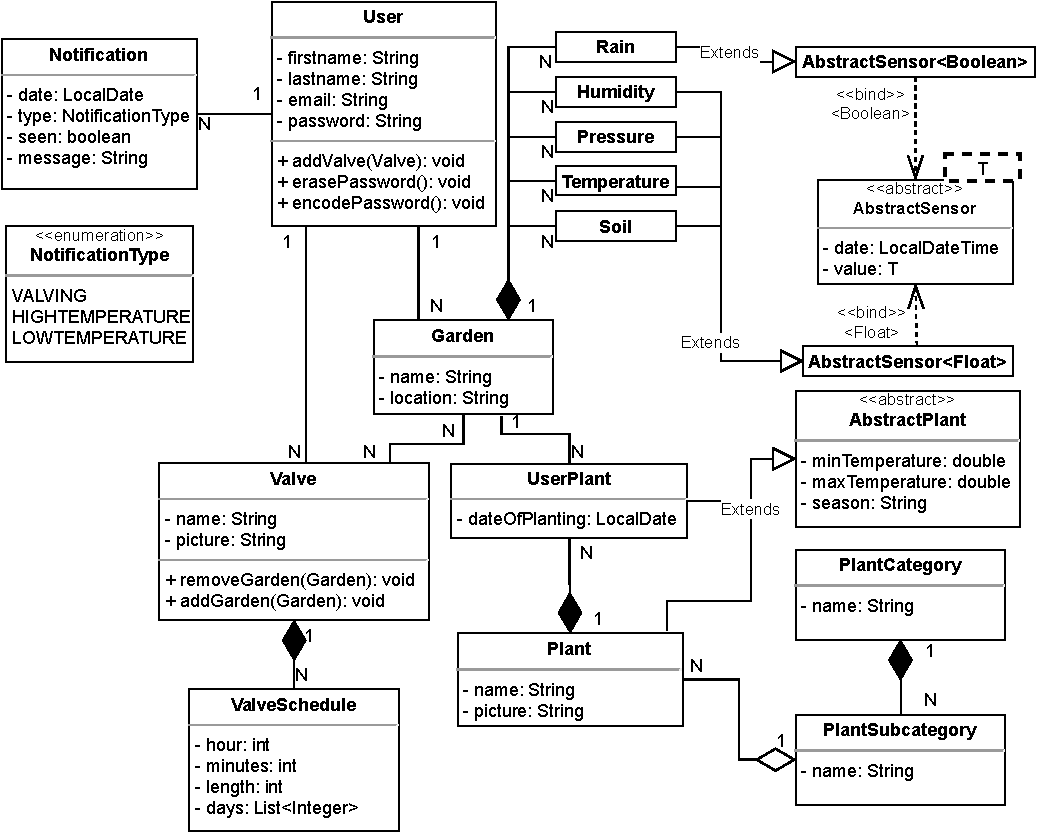
\includegraphics[width= 13 cm, height = 10cm]{ClassDiagram.pdf}
\caption{Diagram tried}
\label{fig:classDiagram}
\end{figure}

\section{Sekvenčný diagram}
\begin{figure}[H]
\includegraphics[width= 13 cm]{SekvencnýDiagram.pdf}
\caption{Sekvenčný diagram}
\label{fig:sequenceDiagram}
\end{figure}

\chapter{Implementácia}
Zvolené implementačné riešenie naväzuje na navrhované riešenie v predchádzajúcej kapitole.

\section{Softvér}
V backendovom riešení aplikácie som zvolila konkrétne framework jazyka Java - Spring Boot, vo frontendovom riešení aplikácie javascriptovú knižnicu React. Podrobný popis použitia je popísaný v nasledujúcich sekciách.

\subsection{Backend}
Pre vývoj backendovej časti aplikácie som zvolila jazyk Spring Boot. Dôvody výberu jazyka Java sú spomenuté v sekcií ~\ref{sec:software}. Konkrétne framework Spring Boot ponúka auto konfiguráciu závislostí, čo uľahčuje prácu pre vývoj v jazyku Java, preto som sa rozhodla pre túto možnosť implementácie.

Jednotlivá práca s dátami a ich úprava sa nachádza práve v Spring Boot aplikácii. Ide o dáta užívateľov, záhrad, rastlín, či senzorov. 

\subsubsection{Získavanie dát zo senzorov}
Spring Boot pre získanie nameraných dát pomocou senzorov komunikuje prostredníctvom AMQP protokolu s RabbitMQ brokerom, ktorý slúži ako nástroj na spracovanie správ. Pomocou anotácie  \textsf{@RabbitListener} Spring dokáže počúvať na jednotlivých poradovníkoch brokera, z ktorých si dokáže brať dáta v momente ich výskytu.

\subsubsection{Dynamický rozvrh}
Požiadavka ktorá znie \textit{"Systém umožní užívateľovi nastaviť čas pravidelného zalievania."} požaduje nastaviť plán zalievania dynamicky, v čase behu aplikácie. Táto požiadavka je vyriešená pomocou dvoch rozvrhových nástrojov. Metóda označená anotáciou \textsf{@Scheduled} sa spustí každú polnoc, kedy vykoná nastavenie jednotlivých dynamických rozvrhov pomocou \textsf{ScheduledExecutorService}. V momente dosiahnutia časového plánu rozvrhu, sa spustí metóda na otočenie ventilového kontroléra a zároveň nastaví kontreléru časovač na jeho uzatvorenie. Pred spustením zalievania sa skontroluje, či je rozvrh stále v databáze pre prípad, že ho užívateľ vymazal v daný deň polievania.

\subsection{Užívateľské rozhranie}
Užívateľské rozhranie je postavené pomocou JavaScriptovej knižnice React.  Konkrétne knižnicu React som si vybrala kvôli jeho flexibilite, ktorá dovoľuje vytváranie znovu použiteľných komponentov a kvôli využívaniu JSX syntaxe, ktorá umožňuje kombinovať HTML s JavaScriptom.


\section{Komunikácia s hardvérom}
Hardvérové komponenty pozostávajú z mikročipu ESP8266, senzorov pre meranie teploty, vlhkosti vzduchu, pôdy, tlaku vzduchu, zrážkomeru a senzoru, ktorý slúži na uzatvorenie ventilov.

\subsection{Mikročip ESP8266}
Mikročip ESP8266 obsahuje implementáciu kódu napísanú v Arduino jazyku, ktorý zabezpečuje pripojenie mikročipu k sieti prostredníctvom wifi prijímača, riadenie senzorov pomocou tohoto mikročipu a komunikáciu mikročipu s RabbitMQ brokerom. Získané dáta zo senzorov následne odosiela pomocou MQTT protokolu na RabbitMQ brokera. Implementácia zahŕňa aj odber príkazov prichádzajúcich z RabbitMQ.

\subsection{Senzory}
Pre senzor BME280, ktorý je použitý na meranie teploty, tlaku a vlhkosti vzduchu, sú v Arduino kóde použité knižnice  <Adafruit\_Sensor.h> a  <Adafruit\_BME280.h>, ktoré poskytujú metódy na komunikáciu so senzorom a rozlišovanie jednotlivých hodnôt nameraných týmto senzorom. Dáta zo zrážkomera prijme mikročip ESP8266 z digitálneho výstupu senzora a dáta namerané senzorom pre vlhkosť pôdy prijme ESP8266 z analógového výstupu senzora.

\subsection{Ventilový kontrolér}
Riadenie uzatvárania ventilu pre prívod vody zabezpečuje Tuya inteligentný ventilový kontrolér. Vďaka zabudovanému wifi prijímaču v kontroléri je možné kontrolér pripojiť do lokálnej siete. Na nakonfigurovanie sieťových prístupových údajov je potrebné stiahnutie Tuya aplikácie. Pre ovládanie kontroléra pomocou API je nutná registrácia na Tuya IoT Development platforme. V tejto platforme je následne nutné nakonfigurovať nastavenia a prepojiť účet s pripojeným zariadením, v tomto prípade účet s ventilovým kontrolérom. V tomto okamihu je možné ovládať zariadenie pomocou API. Spring Boot následne komunikuje s rozhraním, a tak dokáže získať informácie od zariadení v tomto rozhraní, či ovládať ich funkcionalitu. V tomto prípade funkcionalitu kontroléra, ako je pohyb ventilu alebo nastavenie časovača, po ktorom sa tento pohyb ventilu vykoná.

\chapter{Testovanie}

\chapter{Záver}
Cieľom práce bolo vytvoriť prieskum existujúcich riešení, zadefinovať požiadavky na systém a vytvoriť návrh implementácie, čo sa v tejto práci podarilo naplniť. Pre lepšie  pochopenie kontextu, práca obsahuje aj vysvetlenie používaných pojmov. Na túto prácu bude následne naväzovať bakalárska práca, s plánom nasledujúcej implementácie navrhovaného riešenia systému, pripojenie hardvérovej časti k softvérovej časti systému a vytvorenie testovacích scenárov, otestovania aplikácie a následného vyhodnotenia testovania. 

\printindex

\appendix

\begin{thebibliography}{46}
\bibitem{morgan} MORGAN, Jacob. A Simple Explanation Of 'The Internet Of Things'. \textit{Forbes} [online]. 2014 [cit. 2020-10-18]. Dostupné z: https://www.forbes.com/sites/jacobmorgan/2014/05/13/simple-explanation-internet-things-that-anyone-can-understand/\#767942d51d09
\bibitem{economy} ALBARRAN, Alan B. \textit{The Media Economy}. 2nd edition. New York: Routledge, 2017, s.~93. ISBN 9781138886094.
\bibitem{iot}U.FAROOQ, M., Muhammad WASEEM, Sadia MAZHAR, Anjum KHAIRI a Talha KAMAL. A Review on Internet of Things (IoT). \textit{International Journal of Computer Applications} [online]. 2015, \textbf{113}(1), 1-7 [cit. 2020-10-18]. ISSN 09758887. Dostupné z: doi:10.5120/19787-1571
\bibitem{suresh}SURESH, P., J. Vijay DANIEL, V. PARTHASARATHY a R. H. ASWATHY. A state of the art review on the Internet of Things (IoT) history, technology and fields of deployment. In: \textit{2014 International Conference on Science Engineering and Management Research (ICSEMR)}. Chennai: IEEE, 2014, 2014, s.~1-8. ISBN 978-1-4799-7613-3. Dostupné z: doi:10.1109/ICSEMR.2014.7043637
\bibitem{smartcity} ZANELLA, Andrea, Nicola BUI, Angelo CASTELLANI, Lorenzo VANGELISTA a Michele ZORZI. Internet of Things for Smart Cities. In: \textit{IEEE Internet of Things Journal}. IEEE, 2014, s.~22-32. ISSN 2327-4662. Dostupné z: doi:10.1109/JIOT.2014.2306328
\bibitem{smartgrid} FANG, Xi, Satyajayant MISRA, Guoliang XUE a Dejun YANG. \textit{Smart Grid - The New and Improved Power Grid: A Survey}. In: . 2012, s.~944-980. ISSN 1553-877X. Dostupné z: doi:10.1109/SURV.2011.101911.00087
\bibitem{trends}ARSHAD, Rushan, Saman ZAHOOR, Munam Ali SHAH, Abdul WAHID a Hongnian YU. Green IoT: An Investigation on Energy Saving Practices for 2020 and Beyond. In: \textit{IEEE Access}. IEEE, 2017, s.~15667-15681. ISSN 2169-3536. Dostupné z: doi:10.1109/ACCESS.2017.2686092
 \bibitem{homedef}YANG, Lili, Shuang-Hua YANG a Fang YAO. Safety and Security of Remote Monitoring and Control of intelligent Home Environments. \textit{2006 IEEE International Conference on Systems, Man and Cybernetics} [online]. IEEE, 2006, 2006, , 1149-1153 [cit. 2020-10-26]. ISBN 1-4244-0099-6. Dostupné z: doi:10.1109/ICSMC.2006.384555
   \bibitem{azureHub}\textit{IoT Solutions in Microsoft's Azure IoT Suite: Data Acquisition and Analysis in the Real World} [online]. Berkeley, CA: Apress, 2017, s.~41-46 [cit. 2020-11-12]. ISBN 978-1-4842-2143-3. Dostupné z: DOI: 10.1007/978-1-4842-2143-3
  \bibitem{protocols} NAIK, Nitin. Choice of effective messaging protocols for IoT systems: MQTT, CoAP, AMQP and HTTP. In: \textit{2017 IEEE International Systems Engineering Symposium (ISSE)}. Vienna: IEEE, 2017, 2017, s.~1-7. ISBN 978-1-5386-3403-5. Dostupné z: doi:10.1109/SysEng.2017.8088251  
   \bibitem{coap} CoAP - Constrained Application Protocol: Web Protocol for IoT. \textit{Radiocrafts} [online]. Oslo: Radiocrafts, c2003-2020 [cit. 2020-11-14]. Dostupné z: https://radiocrafts.com/technologies/coap-constrained-application-protocol/
    \bibitem{http} BHOLA, Siddharth. Why HTTP is not suitable for IOT applications. In: \textit{Concurrency: Digital Transformation Realized} [online]. Concurrency, c2020, 24 Jun 2019 [cit. 2020-11-14]. Dostupné z: https://www.concurrency.com/blog/june-2019/why-http-is-not-suitable-for-iot-applications
 \bibitem{rabbitmq}AMQP 0-9-1 Model Explained. \textit{Rabbitmq} [online]. VMware, c2007-2020 [cit. 2020-11-14]. Dostupné z: https://www.rabbitmq.com/tutorials/amqp-concepts.html
   \bibitem{PaaS} Co je PaaS?: Platforma jako služba. \textit{Microsoft Azure} [online]. Microsoft [cit. 2020-11-14]. Dostupné z: https://azure.microsoft.com/cs-cz/overview/what-is-paas/   
   \bibitem{iotcloud} PFLANZNER, T. a A. KERTESZ. A survey of IoT cloud providers. In: \textit{2016 39th International Convention on Information and Communication Technology, Electronics and Microelectronics (MIPRO)}. Opatija: IEEE, 2016, 2016, s.~730-735. ISBN 978-953-233-086-1. Dostupné z: doi:10.1109/MIPRO.2016.7522237
 \bibitem{google} Google Cloud IoT solutions. \textit{Google Cloud} [online]. Google [cit. 2020-11-14]. Dostupné z: https://cloud.google.com/solutions/iot/
 \bibitem{heroku} CloudMQTT. \textit{Heroku} [online]. Salesforce, c2020 [cit. 2020-11-14]. Dostupné z: https://elements.heroku.com/addons/cloudmqtt
 \bibitem{IoTHub}AMMAR, Mahmoud, Giovanni RUSSELLO a Bruno CRISPO. Internet of Things: A survey on the security of IoT frameworks. \textit{Journal of Information Security and Applications}. Elsevier, 2018, \textbf{38}, 8-27. ISSN 22142126. Dostupné z: doi:10.1016/j.jisa.2017.11.002
 \bibitem{comunication}OBAIDAT, Mohammad S., Alagan ANPALAGAN a Isaac WOUNGANG, ed. \textit{Handbook of Green Information and Communication Systems}. 2013. Waltham: Elsevier, 2012, s.~43-48. ISBN 9780124158825.
\bibitem{wifi} WANG, Lei, Dunlu PENG a Ting ZHANG. Design of Smart Home System Based on WiFi Smart Plug. \textit{International Journal of Smart Home}. 2015, \textbf{9}(6), 173-182. ISSN 19754094. Dostupné z: doi:10.14257/ijsh.2015.9.6.19
 \bibitem{zigbee} FARAHANI, Shahin. \textit{ZigBee Wireless Networks and Transceivers}. 2008. Burlington: Newnes, 2008, s.~1-5. ISBN 9780080558479.
 \bibitem{health}DAGTAS, S., G. PEKHTERYEV a Z. SAHINOGLU. Multi-Stage Real Time Health Monitoring via ZigBee in Smart Homes. In: \textit{21st International Conference on Advanced Information Networking and Applications Workshops (AINAW'07)}. IEEE, 2007, 2007, s.~782-786. ISBN 978-0-7695-2847-2. Dostupné z: doi:10.1109/AINAW.2007.263
\bibitem{z-wave} KNIGHT, M. How safe is Z-Wave? [Wireless standards]. In: \textit{Computing and Control Engineering}. 2006, s.~18-23. ISSN 0956-3385. Dostupné z: doi:10.1049/cce:20060601
\bibitem{bluetooth}BISDIKIAN, C. An overview of the Bluetooth wireless technology. In: \textit{IEEE Communications Magazine}. IEEE, 2001, s.~86-94. ISSN 0163-6804. Dostupné z: doi:10.1109/35.968817
\bibitem{ble} SIEKKINEN, Matti, Markus HIIENKARI, Jukka K. NURMINEN a Johanna NIEMINEN. How low energy is bluetooth low energy? Comparative measurements with ZigBee/802.15.4. In: \textit{2012 IEEE Wireless Communications and Networking Conference Workshops (WCNCW)}. Paris: IEEE, 2012, 2012, s.~232-237. ISBN 978-1-4673-0682-9. Dostupné z: doi:10.1109/WCNCW.2012.6215496
\bibitem{casio}SORREL, C. Casio Bluetooth Low Energy Watch Has Two Year Battery Life. \textit{Wired magazine} [online]. 2011, 24.03.2011 [cit. 2020-10-27]. Dostupné z: https://www.wired.com/2011/03/casio-bluetooth-low-energy-watch-has-two-year-battery-life/
\bibitem{enocean}LI, Xiaohui, Guang CHEN, Bing ZHAO a Xiaobing LIANG. A kind of intelligent lighting control system using the EnOcean network. In: \textit{2014 International Conference on Computer, Information and Telecommunication Systems (CITS)}. IEEE, 2014, 2014, s.~1-5. ISBN 978-1-4799-4383-8. Dostupné z: doi:10.1109/CITS.2014.6878964
\bibitem{enoceancvut}LÁBAJ, Ondrej, Renata RYBÁROVÁ a Gregor ROZINAJ. \textit{Automatizácia domácnosti}. 2017. Praha: České vysoké učení technické v Praze, 2017. ISBN 978-80-01-06230-2.
  \bibitem{networks}LI JIANG, DA-YOU LIU a BO YANG. Smart home research. In: \textit{Proceedings of 2004 International Conference on Machine Learning and Cybernetics (IEEE Cat. No.04EX826)}. IEEE, 2004, s.~659-663. ISBN 0-7803-8403-2. Dostupné z: doi:10.1109/ICMLC.2004.1382266
 \bibitem{securitytitle}ALI, Waqar, Ghulam DUSTGEER, Muhammad AWAIS a Munam Ali SHAH. IoT based smart home: Security challenges, security requirements and solutions. In: \textit{2017 23rd International Conference on Automation and Computing (ICAC)}. Huddersfield: IEEE, 2017, 2017, s.~1-6. ISBN 978-0-7017-0260-1. Dostupné z: doi:10.23919/IConAC.2017.8082057
\bibitem{security}KOMNINOS, Nikos, Eleni PHILIPPOU a Andreas PITSILLIDES. Survey in Smart Grid and Smart Home Security: Issues, Challenges and Countermeasures. In: \textit{IEEE Communications Surveys \& Tutorials}. Vol.~16. Fourthquarter: IEEE, 2014, s.~1933-1954. ISSN 1553-877X. Dostupné z: doi:10.1109/COMST.2014.2320093
\bibitem{threats}SCHIEFER, Michael. Smart Home Definition and Security Threats. In: \textit{2015 Ninth International Conference on IT Security Incident Management \& IT Forensics}. Magdeburg: IEEE, 2015, 2015, s.~114-118. ISBN 978-1-4799-9902-6. Dostupné z: doi:10.1109/IMF.2015.17
\bibitem{farmbot} \textit{FarmBot} [online]. San Luis Obispo: FarmBot, 2020 [cit. 2020-12-07]. Dostupné z: www.farm.bot
\bibitem{lorawan}LoRaWAN® Agricultural Monitoring Node-to-App Starter Kit. \textit{Ursalink} [online]. Xiamen Ursalink Technology, 2017 [cit. 2020-12-03]. Dostupné z: http://www.ursalink.com/en/lorawan-agricultural-monitoring-starter-kit
\bibitem{klarstein}GrowIt Farm inteligentná domáca záhrada. \textit{Klarstein} [online]. Berlin: Chal-Tec, 2020 [cit. 2020-12-03]. Dostupné z: https://www.klarstein.sk/Moderne-byvanie/Inteligentne-kvetinace/GrowIt-Farm-inteligentna-domaca-zahrada-28-rastlin-48-W-LED-8-litrov-28-rastlin.html?force\_sid=edsf6rt1lgbqithnhi0vtsjkm7
\bibitem{gardena} Smart senzor, zavlažovací počítač - súprava. \textit{Gardena} [online]. GARDENA, 2008 [cit. 2020-12-05]. Dostupné z: www.gardena.com/sk/produkty/zavlaha/riadenie-zavlazovania/smart-senzor-zavlazovaci-pocitac---suprava/967046701/
\bibitem{agrivi} \textit{Agrivi} [online]. Agrivi, 2013 [cit. 2020-12-06]. Dostupné z: https://www.agrivi.com/
\bibitem{planner} \textit{Territorial Seed Company Garden Planner} [online]. Growing Interactive, 2007 [cit. 2020-12-06]. Dostupné z: https://gardenplanner.territorialseed.com
\bibitem{rainbird} \textit{RainBird} [online]. RainBird, 2020 [cit. 2020-12-08]. Dostupné z: https://store.rainbird.com
\bibitem{xiaomimiflora} Xiaomi Mi Flora Monitor - Chytrý senzor pro rostliny. \textit{IStage} [online]. iStage, 2020 [cit. 2020-12-07]. Dostupné z: https://www.istage.cz/chytra-domacnost/xiaomi-mi-flora-monitor-chytry-senzor-pro-rostliny/
\bibitem{agora}IQtech SmartLife Zavírač ventilů voda plyn, VC01W, Wi-Fi. \textit{Agora: dmt} [online]. Brno: CyberSoft, 2020 [cit. 2020-12-12]. Dostupné z: https://www.merkur.agora.cz/iqtech-smartlife-zavirac-ventilu-voda-plyn-vc01w-wi-fi\_d69826.html\#prettyPhoto
\bibitem{conclusionSolution} PATNAIKUNI, Dinkar R Patnaik. A Comparative Study of Arduino, Raspberry Pi and ESP8266 as IoT Development Board. In: \textit{International Journal of Advanced Research in Computer Science}. Vol.~8. Udaipur: International Journal of Advanced Research in Computer Science, 2017, s.~2350-2352. ISSN 09765697. Dostupné z: doi:10.26483/ijarcs.v8i5.3959
\bibitem{esp} \textit{Espressif} [online]. Shanghai: Espressif Systems, 2020 [cit. 2020-12-12]. Dostupné z: www.espressif.com
\bibitem{arduino} \textit{Arduino} [online]. Arduino, 2020 [cit. 2020-12-12]. Dostupné z: https://www.arduino.cc
\bibitem{prosconsArduino} SARWAR, Ismail. Advantages and Disadvantages of Using Arduino. \textit{Engineer Experiences} [online]. Engineer Experiences, 2020, 1 October 2016 [cit. 2020-12-12]. Dostupné z: https://engineerexperiences.com/advantages-and-disadvatages.html
\bibitem{raspberryPi} \textit{Raspberry Pi} [online]. Cambridge: Raspberry Pi [cit. 2020-12-12]. Dostupné z: https://www.raspberrypi.org
\end{thebibliography}


\end{document}